%-------------------------------------------------------------------------------------------------%
% Author: John Joseph Valletta
% Date: 06/03/2015
% Title: Lab sessions
%-------------------------------------------------------------------------------------------------%
% Preamble
%-----------------------------------------------------------------------------%
\documentclass[a4paper,11pt]{article}
\usepackage[top=1.5in, bottom=1.5in, left=1in, right=1in]{geometry}
\usepackage{graphicx}
\usepackage{amsmath}
\usepackage{amssymb}
\usepackage{enumitem}
\usepackage{pdflscape}
\usepackage{framed}
\usepackage[colorlinks=true, urlcolor=blue, linkcolor=black]{hyperref}
\usepackage{color}
\setlength{\parindent}{0pt} % get rid of indentation
\definecolor{dkgreen}{rgb}{0,0.6,0}
\definecolor{gray}{rgb}{0.5,0.5,0.5}
\definecolor{mauve}{rgb}{0.58,0,0.82}
\definecolor{deepblue}{rgb}{0,0,0.5}
\definecolor{deepred}{rgb}{0.6,0,0}
\definecolor{deepgreen}{rgb}{0,0.5,0}
\definecolor{lightgray}{rgb}{0.92,0.92,0.92}
\usepackage{listings}
\newcommand*{\argmin}{\operatornamewithlimits{argmin}\limits}
\newcommand*{\argmax}{\operatornamewithlimits{argmax}\limits}

\lstdefinestyle{RCode}{
language=R,                     % the language of the code
basicstyle=\scriptsize\ttfamily,       % the size of the fonts that are used for the code
numbers=left,                   % where to put the line-numbers
numberstyle=\tiny\color{gray},  % the style that is used for the line-numbers
stepnumber=1,                   % the step between two line-numbers. If it's 1, each line
                          % will be numbered
numbersep=5pt,                  % how far the line-numbers are from the code
backgroundcolor=\color{lightgray},  % choose the background color. You must add \usepackage{color}
showspaces=false,               % show spaces adding particular underscores
showstringspaces=false,         % underline spaces within strings
showtabs=false,                 % show tabs within strings adding particular underscores
frame=lines,%single,                   % adds a frame around the code
rulecolor=\color{black},        % if not set, the frame-color may be changed on line-breaks within not-black text (e.g. commens (green here))
tabsize=2,                      % sets default tabsize to 2 spaces
captionpos=b,                   % sets the caption-position to bottom
breaklines=true,                % sets automatic line breaking
breakatwhitespace=false,        % sets if automatic breaks should only happen at whitespace
title=\lstname,                 % show the filename of files included with \lstinputlisting;
                          % also try caption instead of title
keywordstyle=\color{blue},      % keyword style
commentstyle=\color{dkgreen},   % comment style
stringstyle=\color{mauve},      % string literal style
escapeinside={\%*}{*)},         % if you want to add a comment within your code
morekeywords={}            % if you want to add more keywords to the set
}

%-----------------------------------------------------------------------------%
% Start of document
%-----------------------------------------------------------------------------%
\begin{document}

%-----------------------------------------------------------------------------%
% Title page
%-----------------------------------------------------------------------------%
\begin{center}
{\huge Introduction to Machine Learning for the Life Sciences\\[0.5cm]
Lab Sessions}\\[0.5cm]
by\\[0.5cm]
John Joseph Valletta\\
University of Exeter, Penryn Campus, UK\\[0.5cm]
{\large 1st-2nd June 2015}\\[4cm]
\end{center}
%-----------------------------------------------------------------------------%
% Table of contents
%-----------------------------------------------------------------------------%
%\clearpage
%\tableofcontents
%\clearpage

%-----------------------------------------------------------------------------%
\section*{Introduction}
%-----------------------------------------------------------------------------%
The aim of these lab sessions is to get you started with applying machine learning
algorithms to various types of datasets. The focus is to showcase the versatility of
these methods and give you a flavour of the sort of problems that can be tackled.
We will not be spending time on the topic of \textit{feature extraction}, 
that is, how to extract features which have the best predictive capabilities. This is
usually the crux of any predictive modelling problem but which is domain-specific.
\\\\
We will be using the programming language \textbf{R}, mainly because most life scientists
are already familiar with it, but also because it is an open-source platform that gives you
access to state-of-the-art algorithms. \textbf{Python} (free and extremely 
popular with computer scientists) and \textbf{MATLAB \textsuperscript{\textregistered}} are other
popular choices. You can also find faster implementations in \textbf{C/C++}.
\\\\
These lab sessions are not intended to be an \textbf{R} tutorial. If you want to learn more
about \textbf{R}, please refer to the myriad of free resources available on the web.

\begin{description}[leftmargin=11em,style=nextline]
	\item[Installing R:] \url{http://www.r-project.org/} 
	\item[Installing RStudio:] \url{http://www.rstudio.com/}
\end{description}  

\begin{framed}
\textbf{It is imperative that you read and familiarise yourself with the documentation of 
any machine learning algorithm before using it!} 
\end{framed}

Everyone might have different packages available in their \textbf{R} installation, so
before calling\\ 
{\lstinline[style=RCode, basicstyle=\normalsize\ttfamily] |library(Package Name)|}, please run
{\lstinline[style=RCode, basicstyle=\normalsize\ttfamily] |install.packages("Package Name")|}, where
Package Name is the name of the package you need e.g {\lstinline[style=RCode, basicstyle=\normalsize\ttfamily] |mclust|}

\clearpage
%-----------------------------------------------------------------------------%
\section{Getting started using an artificial dataset}
%-----------------------------------------------------------------------------%
\begin{framed}
\begin{description}[leftmargin=5em,style=nextline]\addtolength{\itemsep}{-0.2\baselineskip}
	\item[Data:] artificial data from a 3D multivariate Gaussian distribution
	\item[Task:] cluster data points (unsupervised)
	\item[Method:] $k$-means and Gaussian mixture models
\end{description} 
\end{framed}

Before starting using real datasets, let us apply some of the algorithms we discussed
to an artificial dataset that we can visualise and control. We will generate 5 sets of data
from a 3-dimensional Gaussian distribution and visualise them.
\vspace{0.3cm}
\begin{lstlisting}[style=RCode]
library(MASS) # mvrnorm (multivariate normal)
library(rgl) # plot3d
N <- 100 # number of data points
sigma2 <- 1 # variance of data points
covMatrix <- sigma2*diag(3) # assume the same variance in all three directions
groupA <- mvrnorm(n=N, mu=c(3, 3, 9), Sigma=covMatrix)
groupB <- mvrnorm(n=N, mu=c(3, 9, 3), Sigma=covMatrix)
groupC <- mvrnorm(n=N, mu=c(9, 9, 9), Sigma=covMatrix)
groupD <- mvrnorm(n=N, mu=c(9, 3, 3), Sigma=covMatrix)
groupE <- mvrnorm(n=N, mu=c(6, 6, 6), Sigma=covMatrix)
xTrain <- rbind(groupA, groupB, groupC, groupD, groupE) # training dataset is 5*N x 3
plot3d(xTrain, col="grey", xlab="x", ylab="y", zlab="z")
\end{lstlisting}
\vspace{-0.2cm}
Visually you can probably deduce that there are 5 different clusters. In practice
however, it is hard to visualise high-dimensional data and we need to resort
to other methods to deduce the number of clusters. 
The main objective of clustering is:

\begin{itemize}
	\item High intra-cluster similarity (points in the same cluster should be similar)
	\item Low inter-cluster similarity (points in distinct clusters should be sufficiently different)
\end{itemize}

To guess the right number of clusters we can run $k$-means several times and plot
the resultant intra- and inter-cluster sum-of-squares as a function of $k$
\vspace{0.3cm}
\begin{lstlisting}[style=RCode]
# k-means, let k vary from 2 to 10
kRange <-  seq(from=2, to=10, by=1)
intraClustSS <- rep(NA, length(kRange))  
interClustSS <- rep(NA, length(kRange))
for (k in kRange){
    fit <- kmeans(x=xTrain, centers=k)
    intraClustSS[k-1] <- fit$tot.withinss # it's (k-1) because k starts from 2
    interClustSS[k-1] <- fit$betweenss
}
minY <- min(c(intraClustSS, interClustSS))
maxY <- max(c(intraClustSS, interClustSS))
plot(kRange, interClustSS, type="o", pch=1, col="blue", lwd=3, lty=1, ylim=c(minY, maxY), xlab="k")
points(kRange, intraClustSS, type="o", pch=1, col="red", lwd=3)
legend("topleft", c("inter-cluster sum-of-squares", "intra-cluster sum-of-squares"), bty="n",
       col=c("blue", "red"), pch=1, lwd=3, lty=1)
\end{lstlisting}

After $k=5$, the sum-of-squares does not change that much, so it can be deduced that
there are 5 distinct clusters in this dataset. Let us visualise the result:
\vspace{0.3cm}
\begin{lstlisting}[style=RCode]
fit <- kmeans(x=xTrain, centers=5)
plot3d(xTrain, col=fit$cluster, xlab="x", ylab="y", zlab="z")
\end{lstlisting}

\begin{framed}
\textbf{Question(s):}
\begin{enumerate}
	\item What happens to the inter/intra-cluster sum-of-squares plot as we increase \texttt{sigma2}?
\end{enumerate}
\end{framed}

Let us perform a similar analysis but using a mixture of Gaussian models, where
we will fit $k$ Gaussians. This time, instead of the inter/intra-cluster sum-of-squares
we will plot the BIC (Bayesian Information Criterion), a goodness-of-fit measure that
penalises model complexity ($k$). The \texttt{Mclust} function uses BIC to decide which
model to retain. To speed up the process we will also tell \texttt{Mclust} that we
want a Gaussian with equal variances in all directions (\texttt{modelNames="EII"}). 
\\
\begin{lstlisting}[style=RCode]
library(mclust) # Gaussian mixture models
fit <- Mclust(data=xTrain, G=seq(10), modelNames="EII")
summary(fit)
plot(fit$BIC, type="o", pch=1, col="blue", lwd=3, lty=1, xlab="k")
legend("topleft", "BIC (Bayesian Information Criterion)", bty="n",
       col=c("blue", "red"), pch=1, lwd=3, lty=1)
plot(fit, what="density", lwd=2)
\end{lstlisting}

\begin{framed}
\textbf{Question(s):}
\begin{enumerate}
	\item Repeat the above but without specifying \texttt{modelNames}. Which model does it retain?
	\item How does the BIC plot and the type of model retained changes when increasing \texttt{sigma2}?
\end{enumerate}
\end{framed}

\clearpage
%-----------------------------------------------------------------------------%
\section{Clustering gene expression data}
%-----------------------------------------------------------------------------%
\begin{framed}
\begin{description}[leftmargin=5em,style=nextline]\addtolength{\itemsep}{-0.2\baselineskip}
	\item[Data:] gene expression \href{http://www.bioconductor.org/packages/release/data/experiment/html/ALL.html}{(data of T- and B-cell Acute Lymphocytic Leukemia)}	
	\item[Task:] deduce the number of distinct phenotypes (unsupervised)
	\item[Method:] agglomerative hierarchical clustering
\end{description} 
\end{framed}

Agglomerative hierarchical clustering is a popular choice in gene expression studies.
The data comes as a $N \times D$ matrix, where $N$ is the number of genes and $D$ is 
the number of biological samples (e.g patients with different medical conditions or 
different tissue samples). The numerical value is a measure of how much the $n$th gene
is expressed for the $d$th biological sample. There are usually two key questions that
can be addressed with clustering:

\begin{enumerate}
	\item Which biological samples exhibit a similar gene expression \textit{signature}?
	\item Which genes vary in a similar fashion?
\end{enumerate} 

Here we will use the popular acute lymphoblastic leukaemia (ALL) dataset. It is a
12625 (genes) $\times$ 128 (patients) microarray dataset. The patients were diagnosed with 
either a B- or T-cell acute lymphocytic leukaemia. Because we have access to the labels 
(type and stage of the disease e.g B2) we can easily assess how well the clustering 
algorithm is doing as we expect the B's and T's to cluster together. Note however 
that class labels are not always available and that the clustering algorithm 
does \textit{not} know what the labels are. It is an unsupervised problem 
(we will turn it into a supervised problem later on).
\\\\
The ALL dataset comes in the form of an {\lstinline[style=RCode, basicstyle=\normalsize\ttfamily] |exprSet|} object,
a data structure used in \href{http://www.bioconductor.org}{Bioconductor}. Bioconductor is
an ensemble of \textbf{R} packages specifically written to analyse high-throughput genomic data.
Let us install Bioconductor (for those who have not got it installed already) and extract
the $N \times D$ gene expression matrix of interest \footnote{Do not worry too much about the details, 
the objective is just to extract the data, but if your work involves this type of data it is 
recommended that you familiarise yourself with Bioconductor}.
\\
\begin{lstlisting}[style=RCode]
source("http://bioconductor.org/biocLite.R") # Install Bioconductor
biocLite() # Install core packages 
biocLite("ALL") # Install the ALL package (takes a few secs)
library(ALL) # Load the ALL package
data(ALL) # Loads ALL dataset to workspace
xTrain <- exprs(ALL) # Extract the 12625 x 128 dataset
colnames(xTrain) <- ALL$BT # Replace patient ID by disease stage to assess clustering
\end{lstlisting}
\vspace{-0.3cm}
For the purpose of this exercise, let us just focus on clustering the 128 patients:
\vspace{0.3cm}
\begin{lstlisting}[style=RCode]
distance <- dist(as.matrix(t(xTrain), method="euclidean")) # Distance between patients
# Perform agglomerative hierarchical clustering using the "complete" linkage function
fit <- hclust(distance, method="complete") 
plot(fit, cex=0.5) # Visualise the resultant dendrogram 
\end{lstlisting}

\begin{framed}
\textbf{Question(s):}
\begin{enumerate}
	\item Keep the distance method fixed and change the linkage method (e.g single, average). What happens to the dendrogram? 
	\item Keep the linkage method fixed and change the distance method (e.g manhattan, minkowski). What happens to the dendrogram?
	\item Try using a correlation distance metric and repeat the above. 
	\\
	\textit{Hint}:
	\begin{lstlisting}[style=RCode, backgroundcolor=\color{white}]
	distmethod <- function(x) as.dist(1-cor(x))
	distance <- distmethod(xTrain)
	\end{lstlisting}
	\vspace{-0.5cm} % I don't know why it was adding so much space before end of box so a little hack
\end{enumerate}
\end{framed}

\clearpage
%-----------------------------------------------------------------------------%
\section{Species distribution modelling}
%-----------------------------------------------------------------------------%
\begin{framed}
\begin{description}[leftmargin=5em,style=nextline]\addtolength{\itemsep}{-0.2\baselineskip}
	\item[Data:] \textit{Bradypus variegatus} (brown-throated slot) geographic distribution data (\href{http://www.cs.princeton.edu/~schapire/maxent/}{Phillips et al. (2006)})	
	\item[Task:] produce a map showing the likely geographic distribution of \textit{Bradypus variegatus} (unsupervised)
	\item[Method:] Gaussian mixture models
\end{description} 
\end{framed}

An ubiquitous challenge in conservation biology is to produce species distribution maps. The objective
is to show how in different regions there is more or less chance of observing the species under consideration.
The dataset consists of 116 latitude and longitude recordings of where \textit{Bradypus variegatus} was observed.
This is a classic density estimation problem which in this case is equivalent to a 2D histogram. Let us start by 
retrieving the dataset which is found in the \texttt{dismo} package and plot a point for every observation. 
\\\\
\begin{lstlisting}[style=RCode]
library(raster) # functions for gridded spatial data
library(dismo) # package containing the Bradypus variegatus dataset
library(rworldmap) # access to map of the world
dataPath <- file.path(system.file(package="dismo"), "ex") # path to data location
bradypusFilePath <- file.path(dataPath, "bradypus.csv") # path to Bradypus dataset
data <-  read.table(file=bradypusFilePath, header=T, sep=",", skip=0) # read data
worldMap <- getMap(resolution = "low") # access world map, xlim = long, ylim = lat
plot(worldMap, xlim = c(-85, -40), ylim = c(-25, 20), asp = 1, axes=T) 
points(data[, 2], data[, 3], pch=20, col="blue", cex=0.5) # add observed data points
\end{lstlisting}

The question now is which variables should we use to fit this histogram. A na\"{i}ve approach is to use the
observed latitude and longitude, after all we would expect to find the same species within short geographical 
distances from where we have already observed some. This approach however ignores the habitat properties
inhabited by \textit{Bradypus variegatus}. A better method would be to use environmental variables (e.g temperature and precipitation), 
which characterise the species' habitat, to fit this distribution, and then convert back to the 
latitude/longitude domain. The \texttt{dismo} package contains a number of bioclimatic variables stored as 
GRD files. This is a popular file format used in GIS (Geographic Information System) and contains grid cell
values for that variable. The naming convention for these variables can be found \href{http://www.worldclim.org/bioclim}{here}
\footnote{Note that temperature data is stored as $^\circ$C $\times 10$ as discussed \href{http://www.worldclim.org/formats}{here}}.	   
The data resolution is $0.5^\circ \times 0.5^\circ$ which is sufficient for illustrative purposes.
The steps taken in this task look something like this:

\clearpage

\begin{enumerate}
	\item Read in and plot environmental variables which cover the geographical area of interest.
	\vspace{0.3cm}
	\begin{lstlisting}[style=RCode]
	grdFiles <- list.files(path=dataPath, pattern='grd', full.names=T) # read path of all .grd files
	envData <- stack(grdFiles) # stack all environmental variables
	plot(envData) # plot to confirm data is OK
	\end{lstlisting}
	\vspace{-0.6cm}

	\item For every observed data point, i.e 116 lat/long positions, extract a value for the environmental variable.\\
	i.e (temperature, precipitation$\ldots$)=$f($latitude, longitude)
	\vspace{0.3cm}
	\begin{lstlisting}[style=RCode]
	xTrain <- extract(envData, data[, 2:3]) # columns 2 (longitude) and 3 (latitude)
	\end{lstlisting}
	\vspace{-0.6cm}

	\item Standardise the environmental data as ranges vary widely.\\ 
	i.e $x_{\mathrm{standardise}} = \frac{x-\mu}{\sigma}$\\
	This is a very important step and if omitted the algorithm might fail to converge
	\vspace{0.3cm}
	\begin{lstlisting}[style=RCode]
	meanXTrain <- apply(xTrain, 2, mean) # compute mean of every column
	sdXTrain <- apply(xTrain, 2, sd) # compute sd of every column
	xTrain <- sweep(xTrain, 2, meanXTrain, FUN="-") # x - mean
	xTrain <- sweep(xTrain, 2, sdXTrain, FUN="/") # (x - mean)/sigma
	\end{lstlisting}
	\vspace{-0.6cm}

	\item Fit a distribution to the standardised data using Gaussian mixture models. Instead of using all 9 variables
	however, only a subset of 3 are considered. The reasons are twofold: i) some variables are highly correlated with each other
	(e.g mean annual temperature and maximum temperature of warmest month), but most importantly because of ii) the \textit{curse of dimensionality}.
	The more variables (dimensions) are considered the more the space will be sparsely populated, unless dataset is extremely large. 
	\vspace{0.3cm}
	\begin{lstlisting}[style=RCode]
	library(mclust)
	envVariables <- c("bio1","bio12", "biome") # chosen environmental variables
	fit <- densityMclust(data=xTrain[, envVariables]) # fit distribution
	\end{lstlisting}
	\vspace{-0.6cm}

	\item Compute the value of the fitted distribution for every geographical grid of interest and plot the species geographical distribution map.
	\vspace{0.3cm}
	\begin{lstlisting}[style=RCode]
	# Standardise test data (xTest is the whole grid not just the 116 obs.)
	xTest <- as.data.frame(subset(envData, subset=envVariables)) 
	xTest <- sweep(xTest, 2, meanXTrain[envVariables], FUN="-")
	xTest <- sweep(xTest, 2, sdXTrain[envVariables], FUN="/")
	# Read the distribution at the test points
	notNA <- complete.cases(xTest) # ignore sea points (NA = sea) 
	pred <- rep(NA, dim(xTest)[1])
	pred[notNA] <- predict(fit, newdata=xTest[notNA, ])
	# Create a data frame with values for the distribution for every grid cell
	df <- data.frame(pred=as.matrix(pred, nrow=nrow(envData), ncol=ncol(envData)))
	coordinates(df) <- coordinates(envData) # set spatial coordinates
	gridded(df) <- TRUE # coerce to SpatialPixelsDataFrame
	rasterDF <- raster(df) # coerce to raster
	library(RColorBrewer) # package for pretty colour palettes
	plot(rasterDF, col=brewer.pal(n=9, name="Reds"))
	points(data[, 2], data[, 3], pch=20, col="blue", cex=0.5) # add observations
	\end{lstlisting}
	\vspace{-0.6cm}

\end{enumerate}

\begin{framed}
\textbf{Question(s):}
\begin{enumerate}
	\item Compare your geographical distribution map to \href{http://www.cs.princeton.edu/~schapire/papers/ecolmod.pdf}{Phillips et al. (2006) pg. 252.} 
	Do you think that a Gaussian mixture model is appropriate for this problem?
	\item Pick different combinations of \texttt{envVariables} and describe how the species distribution map changes. Try also single environmental variables.
\end{enumerate}
\end{framed}

\clearpage

%-----------------------------------------------------------------------------%
\section{Predicting forest cover type from cartographic attributes}
%-----------------------------------------------------------------------------%
\begin{framed}
\begin{description}[leftmargin=5em,style=nextline]\addtolength{\itemsep}{-0.2\baselineskip}
	\item[Data:] forest cover type \href{https://archive.ics.uci.edu/ml/datasets/Covertype}{(UC Irvine Machine Learning Repository)}	
	\item[Task:] predict forest cover type for a set of cartographic measurements (supervised)
	\item[Method:] decision trees and random forests
\end{description} 
\end{framed}

This problem appeared as a competition on \href{http://www.kaggle.com/c/forest-cover-type-prediction}{Kaggle}.
It is a multi-class problem where several cartographic attributes are used to predict the forest cover type.
Data comes from the Roosevelt National Forest of northern Colorado and each row represents an observation 
over a 30m $\times$ 30m  patch. The seven distinct forest cover types (\texttt{Cover Type}) are:

\begin{enumerate}\addtolength{\itemsep}{-0.3\baselineskip}
	\item Spruce/Fir
	\item Lodgepole Pine
	\item Ponderosa Pine
	\item Cottonwood/Willow
	\item Aspen
	\item Douglas-fir
	\item Krummholz
\end{enumerate}

The cartographic attributes are:

\begin{description}[leftmargin=0em,style=nextline]\addtolength{\itemsep}{-0.3\baselineskip}
	\item[\texttt{Elevation}]Elevation in meters
	\item[\texttt{Aspect}]Aspect in degrees azimuth
	\item[\texttt{Slope}]Slope in degrees
	\item[\texttt{Horizontal Distance To Hydrology}]Horizontal distance to nearest surface water features
	\item[\texttt{Vertical Distance To Hydrology}]Vertical distance to nearest surface water features
	\item[\texttt{Horizontal Distance To Roadways}]Horizontal distance to nearest roadway
	\item[\texttt{Hillshade 9am}\footnote{Hillshade index takes an integer value from 0 (complete shadow) to 255 (full sunlight)}]Hillshade index at 9am, summer solstice
	\item[\texttt{Hillshade Noon}]Hillshade index at noon, summer solstice
	\item[\texttt{Hillshade 3pm}]Hillshade index at 3pm, summer solstice
	\item[\texttt{Horizontal Distance To Fire Points}]Horizontal distance to nearest wildfire ignition points
	\item[\texttt{Wilderness Area}]4 binary columns (0 = absence or 1 = presence) of wilderness area designation
	\item[\texttt{Soil Type}]40 binary columns (0 = absence or 1 = presence) of soil type designation
\end{description}

For information on wilderness area designation and soil type please check \href{https://archive.ics.uci.edu/ml/machine-learning-databases/covtype/covtype.info}{additional information},
however it is not essential for the purpose of this exercise. Let us start by reading the 
dataset\footnote{For convenience I have uploaded it to Dropbox where it can be easily accessed using the \texttt{RCurl} package} in and split it into a training and testing dataset.
\\
\begin{lstlisting}[style=RCode]
library(RCurl) # To compose general HTTP requests
options(RCurlOptions = list(capath = system.file("CurlSSL", "cacert.pem", package = "RCurl"), ssl.verifypeer = FALSE)) # To avoid SSL certificate problem
dataPath <- getURL("https://dl.dropboxusercontent.com/u/57002389/ML_Life_Sciences/Data/ForestCoverData.csv") # Location of dataset
data <- read.table(text=dataPath, header=T, sep=",", skip=0) # Use a text connection
data <- data[complete.cases(data), ] # Only 2 cases of missing data so ignore
data$Cover_Type <- factor(data$Cover_Type)
NTOTAL <- dim(data)[1] # Total number of observations
NTRAIN <- 12000 # Let us use this many training datapoints
set.seed(101) # Just so we can reproduce results
trainIndices <- sample(x=NTOTAL, size=NTRAIN, replace=FALSE) 
\end{lstlisting}

Fit a simple decision tree to the data.
\\
\begin{lstlisting}[style=RCode]
library(rpart)
library(rpart.plot)
library(rattle) # For fancyRpartPlot to plot rpart tree nicely
fit <- rpart(Cover_Type ~ ., data=data, subset=trainIndices, method="class")
fancyRpartPlot(fit) # Plot decision tree
predClass = predict(fit, type="class") # Pred class on training dataset
confusionMatrix <- table(data$Cover_Type[trainIndices], predClass)
classError <- 1 - diag(prop.table(confusionMatrix, 1)) # Compute misclassification rates
\end{lstlisting}

Results not promising, especially for \texttt{Cover Type} 4 to 7. Let
us use a Random Forest and see how the \texttt{classError} changes. 
\\
\begin{lstlisting}[style=RCode]
library(randomForest)
fit <- randomForest(Cover_Type ~ ., data=data, subset=trainIndices, ntree=200, importance=TRUE) # Takes a few secs
fit$confusion # Confusion matrix
\end{lstlisting}

The misclassification rate has improved, but for some \texttt{Cover Type} it is still unsatisfactory,
why? A quick look at the confusion matrix reveals how our training dataset is \textit{unbalanced}. 
\texttt{Cover Type} 1 and 2 comprise 85\% of the training examples. Having one class more prevalent
in a dataset is a common problem in classification, for example, you may have lots of data
for healthy people but only a few for those suffering from a particular disease. There are two
approaches to circumvent such problem:

\begin{enumerate}
	\item \textbf{On a data level}: Data is balanced by under/over-sampling the original dataset. The aim is to get roughly
	equal number of classes in the training dataset
	\item \textbf{On an algorithm level}: This depends on the algorithm used, but usually involves adjusting some objective function 
	or specifying directly the class prior
\end{enumerate}

\begin{framed}
\textbf{Question(s):}
\begin{enumerate}
	\item Choose a training dataset that have roughly equal number of classes and repeat the fitting process (both a simple decision tree 
	and Random Forest). What is the model's performance now? (compute misclassification error rates for both \textit{training} and \textit{testing} datasets)
	\\
	\textit{Hint}: \texttt{predClass <- predict(fit, newdata=data[-trainIndices, ])}
	\item Repeat the above, but instead of balancing the dataset, specify the class prior by setting the \texttt{classwt} in the \texttt{randomForest} function.
	How does the model's performance compare with the above?
	\item Using the model which gave you the best performance, can you elucidate on the most important variables? 
	\\
	\textit{Hint}: Plot the variable importance plot \texttt{varImpPlot(fit)} 
	\item Instead of having 40 binary columns for \texttt{Soil Type} how else can you ``code'' this variable?
\end{enumerate}
\end{framed}

\clearpage
%-----------------------------------------------------------------------------%
\section{Classifying patients by their gene expression signature}
%-----------------------------------------------------------------------------%
\begin{framed}
\begin{description}[leftmargin=5em,style=nextline]\addtolength{\itemsep}{-0.2\baselineskip}
	\item[Data:] gene expression \href{http://www.bioconductor.org/packages/release/data/experiment/html/ALL.html}{(data of T- and B-cell Acute Lymphocytic Leukemia)}	
	\item[Task:] predict a patient's phenotype using their gene expression signature (supervised)
	\item[Method:] decision trees
\end{description} 
\end{framed}

Here we will consider again the gene expression data from the previous clustering exercise. This
time however we formulate it as a supervised learning problem. Given a gene expression signature
can we predict the patient's phenotype? Let us start by considering only a binary classifier, that is,
discriminating between B- and T-cell cancer types. As this is an illustrative example and the sample 
size is fairly small let us use all available data for training\footnote{Note that if we do this, we cannot infer the generalisation error.
In this case using cross-validation would have been a more sensible option, but this was not discussed in detail in the workshop}.
\\
\begin{lstlisting}[style=RCode]
library(ALL) # Load the ALL package
data(ALL) # Loads ALL dataset to workspace
xTrain <- t(exprs(ALL)) # Extract the 128 x 12625 dataset
yTrain <- factor(substr(ALL$BT,1,1)) # Class is either B or T
df <- data.frame(x=xTrain, y=yTrain) # Create a data frame, x - all inputs, y - class
\end{lstlisting}

\begin{framed}
\textbf{Question(s):}
\begin{enumerate}
	\item Try logistic regression, a very popular statistical binary classifier
	\\
	\textit{Hint}: {\lstinline[style=RCode, basicstyle=\normalsize\ttfamily] |glm(y ~ ., data=df, family=binomial(link="logit")))|}
	\\
	What's the outcome and why?
	\item Use decision trees now
	\\
	\textit{Hint}: use the same code as listed in the previous Forest Cover Type exercise 
	\\
	What's the classifier's performance on the training dataset?
	\item Repeat the above but now we want to infer the stage of the disease as well
	\\
	\textit{Hint}: Set {\lstinline[style=RCode, basicstyle=\normalsize\ttfamily] |yTrain <- factor(ALL$BT)|}
	\vspace{-0.5cm} % I don't know why it was adding so much space before end of box so a little hack
\end{enumerate}
\end{framed}

\clearpage
%-----------------------------------------------------------------------------%
\section{Identifying patients with Parkinsons's disease from speech recordings}
%-----------------------------------------------------------------------------%
\begin{framed}
\begin{description}[leftmargin=5em,style=nextline]\addtolength{\itemsep}{-0.2\baselineskip}
	\item[Data:] audio recordings \href{https://archive.ics.uci.edu/ml/datasets/Parkinsons}{(UC Irvine Machine Learning Repository)}	
	\item[Task:] predict presence of Parkinson's disease (supervised)
	\item[Method:] support vector machine (SVM)
\end{description} 
\end{framed}

Parkinson's disease is a neurological condition that affects millions of people and their families. Around 90\% of 
people with Parkinson's show some form of speech impairment. The premise of this study is to use audio recordings
from a sustained phonations experiment\footnote{Patient is asked to produce and sustain a single vowel at constant pitch}
to classify patients as having Parkinson's or not; a binary classification problem. A total of 22 features (predictors), metrics
related to the frequency content of the audio signal, were extracted from 195 recordings\footnote{For further information on how these 
metrics were computed please refer to \href{http://www.ncbi.nlm.nih.gov/pmc/articles/PMC3051371/}{Little et al. (2009)} but it is not essential for the purpose of this exercise}.
Let us load the dataset and scale all 22 features (feature scaling) to be in the -1 to +1 range ($x' = \frac{2(x - x_{\mathrm{min}})}{(x_{\mathrm{max}}-x_{\mathrm{min}})}-1$). 
The variable \texttt{status} is 0 or 1 indicating absence or presence of disease. 
\\
\begin{lstlisting}[style=RCode]
library(RCurl) # To compose general HTTP requests
options(RCurlOptions = list(capath = system.file("CurlSSL", "cacert.pem", package = "RCurl"), ssl.verifypeer = FALSE)) # To avoid SSL certificate problem 
dataPath <- getURL("https://archive.ics.uci.edu/ml/machine-learning-databases/parkinsons/parkinsons.data") # Location of dataset
data <- read.table(text=dataPath, header=T, sep=",", skip=0, row.names=1) # Text read
data$status <- factor(data$status) # Convert to factor (0/1) (disease absence/presence)
iiPredictors <- which(names(data)!="status") # Column number for all (22) predictors
# Scale all features to -1 to +1 (all data columns except "status")
# x' = 2*(x - xmin)/(xmax - xmin) - 1
xMin <- apply(data[, iiPredictors], 2, min)
xMax <- apply(data[, iiPredictors], 2, max)
# Feature scaling
data[, iiPredictors] <- sweep(data[, iiPredictors], 2, xMin, FUN="-")
data[, iiPredictors] <- 2*data[, iiPredictors]
data[, iiPredictors] <- sweep(data[, iiPredictors], 2, (xMax-xMin), FUN="/")
data[, iiPredictors] <- data[, iiPredictors] - 1
\end{lstlisting}

Next we will split the data into a training (60\%) and testing (40\%) set. The testing dataset will
be used to estimate the generalisation performance of the model. Apart from the misclassification
rates and because we are dealing with a binary classification problem, we will also display the results 
as a receiver operating characteristic (ROC) curve. The various definitions (true positive, true negative etc...)
are depicted in Figure \ref{fig:DefinitionsPlot}.
\clearpage
\begin{lstlisting}[style=RCode]
#--------------------------------------------------------------------------------------#
# Split into training/testing 60% - 40%
set.seed(101) # Just so we can reproduce results
trainIndices <- sample(x=dim(data)[1], size=round(dim(data)[1]*0.6), replace=FALSE)
#--------------------------------------------------------------------------------------#
# Train SVM
library(e1071) # A support vector machine (SVM) library (there is also kernlab)
fit <- svm(status ~., data=data, subset=trainIndices, type="C-classification", kernel="linear", probability=TRUE)
#--------------------------------------------------------------------------------------#
# Compute misclassification rates on testing dataset
predClass <- predict(fit, newdata=data[-trainIndices, ], type="class") # 0/1
confusionMatrix <- table(data$status[-trainIndices], predClass)
classError <- 1 - diag(prop.table(confusionMatrix, 1))
#--------------------------------------------------------------------------------------#
# Plot Receiver operating characteristic (ROC)
library(ROCR) # ROC curves library
# Compute prediction probabilities rather than just class
predProb <- predict(fit, newdata=data[-trainIndices, ], probability=TRUE)
# Prediction object needed by ROCR
# prediction(probability of class=positive class, actual class label)
predObj <- prediction(attr(predProb, "probabilities")[, 1], data$status[-trainIndices]) 
ROCObj <- performance(predObj, "tpr", "fpr") # ROC object
plot(ROCObj) # Plot false positive rate vs true positive rate
abline(a=0, b=1, col="red", lty=2) # Randomly guessing line
#--------------------------------------------------------------------------------------#
# Compute area under ROC curve (AUC)
# AUC = 0.5 (randomly guessing class), AUC = 1 (perfect predictor)
areaUnderCurve <- performance(predObj, "auc") # Compute AUC
areaUnderCurve <- unlist(slot(areaUnderCurve, "y.values")) # Extract AUC (converting S4 class to vector)
\end{lstlisting}

%------------------------------------------------------------------%
\begin{figure}[htbp]
	\centering
	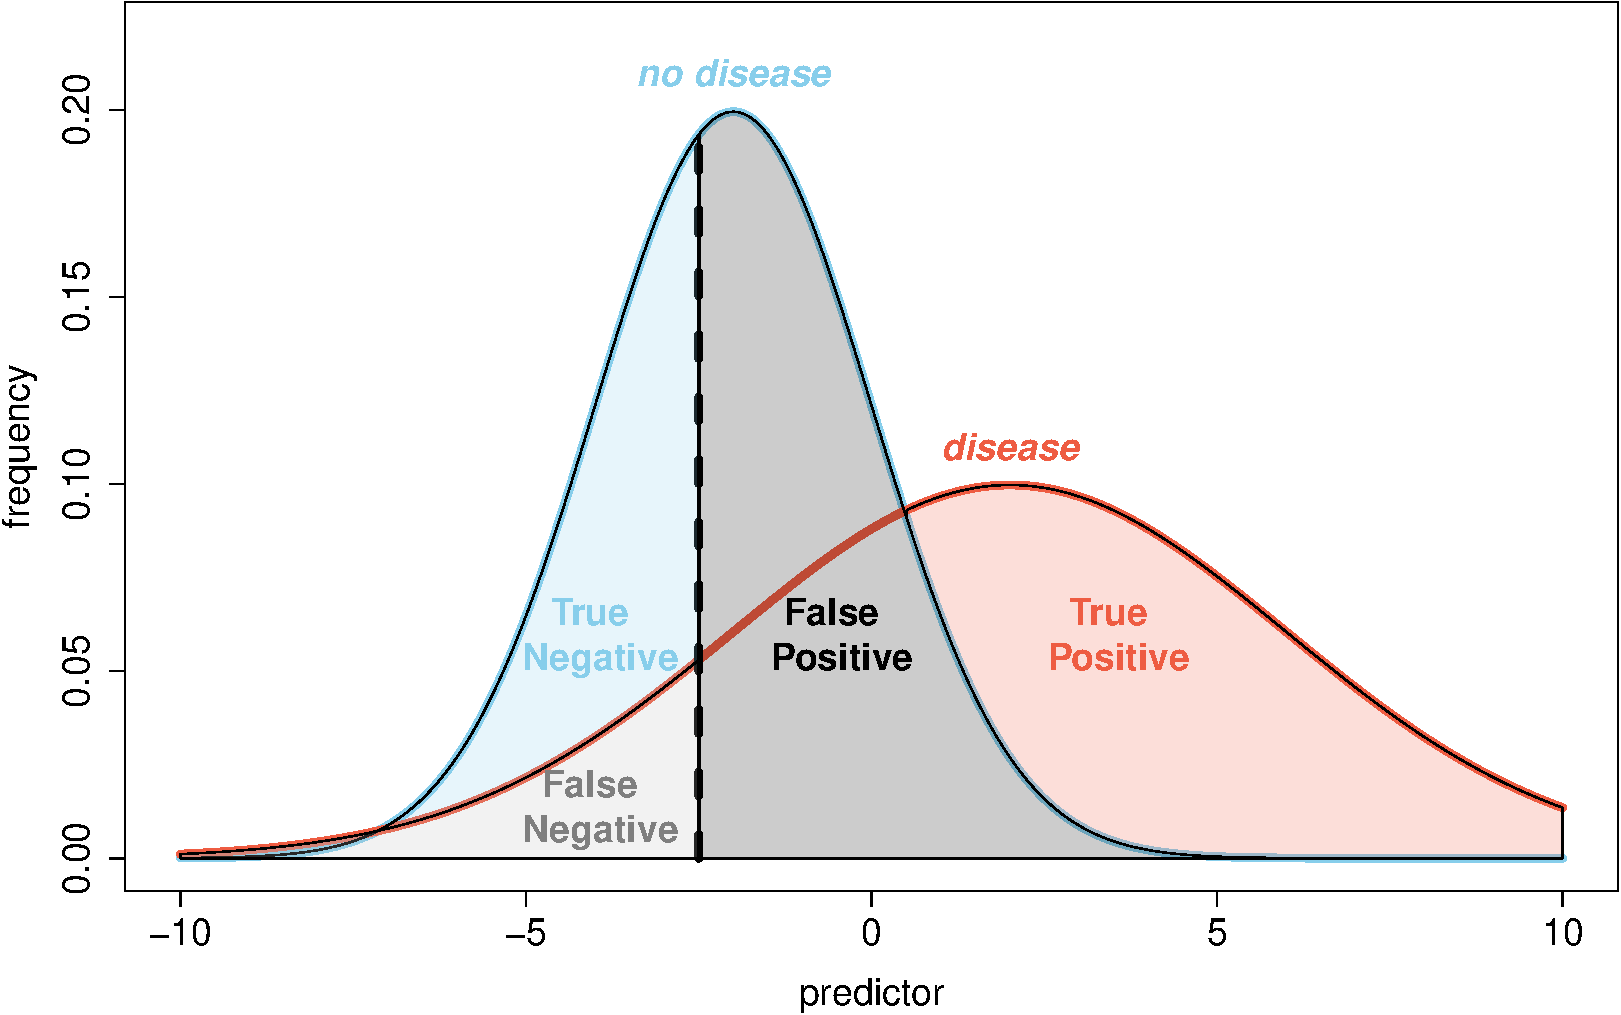
\includegraphics[width=0.8\textwidth]{DefinitionsPlot.pdf}
	\caption{Binary classification definitions for a hypothetical predictor with a class cut-off depicted by the dotted black line}
	\label{fig:DefinitionsPlot}
\end{figure}
%------------------------------------------------------------------%

\begin{framed}
\textbf{Question(s):}
\begin{enumerate}
	\item Why is the misclassification rate of the ``no disease" class much worse than the ``disease" class? What can we do?
	\item Can we reduce the number of predictors \textit{without} taking into consideration the output class (unsupervised feature selection)? 
	\\
	\textit{Hint}: In this case, because all the predictors for an observation were derived from the \textit{same} audio recording, 
	we can deduce that some metrics are highly correlated and thus introducing no further knowledge to our dataset
	\\
	\begin{lstlisting}[style=RCode, backgroundcolor=\color{white}]
	library(corrgram)
	corrgram(data[, iiPredictors], lower.panel=panel.shade, upper.panel=panel.conf)
	\end{lstlisting}
	\vspace{-0.6cm} % I don't know why it was adding so much space before end of box so a little hack
	\item Repeat the analysis and compare results when using the reduced feature set, and also for the case of a radial basis function kernel 
	\\
	\textit{Hint}: Use {\lstinline[style=RCode, basicstyle=\normalsize\ttfamily] |kernel="radial"|}
	\vspace{-0.5cm} % I don't know why it was adding so much space before end of box so a little hack
\end{enumerate}
\end{framed}

%-----------------------------------------------------------------------------%
% End of document
%-----------------------------------------------------------------------------%
\end{document}